\chapter{Introduction}
\thispagestyle{fancy}
\bigskip Multicollinearity is a well-known problem in regression analysis~\cite{gujarati2009basic} and refers to the existence of a perfectly linear relationship or high correlation between multiple independent variables~\cite{gujarati2009basic}. When regression analysis is applied to analyze the effects of independent variables, the regression coefficients of some independent variables exhibiting multicollinearity may be biased. 
% \song{how does it affect other non-regression classifiers?}
Besides, it affects the interpretability of the variable importance measure when using non-regression models such as random forest and decision tree~\cite{Laura2011BioinformaticsClassification, Strobl2008BMCConditional}. Therefore, multicollinearity is generally removed to facilitate regression analysis~\cite{gujarati2009basic}.

Multicollinearity is also observed for various software metrics used for defect prediction studies~\cite{Emam2001TSEconfoundingeffect}. As software metrics usually measure the complexity of software and its development process, many metrics are linearly correlated~\cite{Khoshgoftaar1990developmenterrors}.
Van Koten et al. reported that the multicollinearity in software metrics can cause the stability issue of multiple linear regression models~\cite{VanKoten2006ISTmaintainability}.
%Existing study showed that the multicollinearity in software metrics can cause the stability issue of {\em multiple linear regression models}~\cite{VanKoten2006ISTmaintainability}. 
%Since multicollinearity is considered generally harmful, 
Along this line, many defect prediction studies also consider that multicollinearity should be removed to build better prediction models by using feature extraction, e.g., principal component analysis (PCA)~\cite{Zhang2017TSEaggregate} or feature selection, variance inflation factor (VIF), clustering variable (VC), removal of redundant metrics (RR), manual feature selection (MFS), and stepwise variable selection (SVS)
%\song{list the detailed FS approaches?}
~\cite{Kamei2013TSEjit,Taba2013ICSMantipattern,Lee2016TSEMIM,Kamei2016EMSEjit}.
%For example, principal component analysis (PCA) has been widely used to remove multicollinearity~\cite{Zhang2017TSEaggregate}.
%Van Koten et al. pointed out that multicollinearity can cause the stability issue of {\em multiple linear regression models}~\cite{VanKoten2006ISTmaintainability}.

However, the multicollinearity issue was not explicitly resolved in some defect prediction studies~\cite{Rahman2014ICSEpredictionfinder, Nam2015FSEHDP, Xia2016TSEHydra}. For example, to maximize prediction performance, Rahman et al.~\cite{Rahman2014ICSEpredictionfinder} intentionally used all available software metrics rather than addressing the multicollinearity. This contradictory research trend is not well discussed in the literature.
%However, in the literature, a large number of defect prediction studies did not explicitly handle the multicollinearity issue in software metrics~\cite{Rahman2014ICSEpredictionfinder,Nam2015FSEHDP,Xia2016TSEHydra,Wang2016ICSEsemantic,Muller2016ICSEbiometric,Tantithamthavorn2017TSEcomparemodels}. To maximize prediction performance, most of these studies used all available software metrics without addressing the multicollinearity issue.%~\cite{Rahman2014ICSEpredictionfinder}.This contradictory research trend is not well discussed in the literature. 
Yet, little is known about the performance impact of multicollinearity in software defect prediction practice.
%\emph{Do we need to remove multicollinearity of software metric data to build defect prediction models?} Without answering this question, it is not clear that removing multicollinearity is always necessary. 
%It is also not clear that the studies that did not resolve the multicollinearity issue simply ignore the issue without being aware.


In this sense, the goal of this study is to investigate the impact of the multicollinearity and provide practical guidelines for handling the multicollinearity problem in defect prediction studies. 
To achieve the goal, we first discuss the multicollinearity problem from a theoretical perspective. 
Then, handling of this problem in previous studies is considered, with relevant works being surveyed and categorized.
Focusing on defect prediction performance, we conduct an empirical study to investigate the effect of multicollinearity. Covering 11 different types of existing model from literature, we conducted a total of 1,485,000 predictions.
%Then, we surveyed and categorized previous studies to investigate how the multicollinearity issue was handled. We also conducted an empirical study to investigate how multicollinearity affects defect prediction performance. 
% we discussed the multicollinearity issue theoretically and conducted a large scale empirical study.\jc{as I updated abstract, also say we conducted a survey.} 
% In our empirical study, we built xxx\jc{update} prediction models based on 12 approaches to investigate the effect of multicollinearity on 14 datasets from AEEEM, Relink, JIT\textunderscore QA software projects.
% In our empirical study, we built 48\jc{need to put actual number of models built by your tool by considering repeation and the number of folds to show our study is reall a large scale.} prediction models based on 12 different approaches to investigate the impact of the multicollinearity on 14 datasets from AEEEM, Relink, and JIT\textunderscore QA software projects\jc{cite for each dataset name}.
Then, the effects of multicollinearity on 45 datasets from AEEEM, ReLink, JIT\textunderscore QA, NASA, and PROMISE group~\cite{DAmbros2012EMSEbenchmark, Wu2011FSEReLink, Kamei2013TSEjit, ghotra2017msr} are examined. The results show that defect prediction performance is not always improved by multicollinearity removal techniques such as PCA, VIF, variable clustering and removal of redundant metrics (VCRR). 
% However, correlation-based feature selection (CFS)-BestFirst, a feature selection approach that does not perfectly remove multicollinearity, exhibits the best performance, with statistical significance. Similar results are obtained under various settings. 
Thus, we conclude that multicollinearity removal is not necessary to improve defect prediction performance; however, appropriate consideration of the research objectives is necessary. 
% In our empirical study, we build  117,000 prediction models based on 13 different approaches to investigate the impact of the multicollinearity on 45 datasets from AEEEM, Relink, and JIT\textunderscore QA, NASA, and PROMISE group~\cite{DAmbros2012EMSEbenchmark, Wu2011FSEReLink, Kamei2013TSEjit, ghotra2017msr}.
% \jc{cite for each dataset name}.
% \todo{to be updated when we have the final results} 
% Our experimental results show that PCA and VIF\song{need VIF's full name here, if nesscessary we can intro these two different approaches in the first paragraph of Introduction} techniques which remove the multicollinearity of datasets do not always increase the performance of defect prediction. 
% Our experimental results show that Principal Component Analysis (PCA), Variance Inflation Factor (VIF), and Variable Clustering and removal of redundant metrics (VCRR) technique which remove the multicollinearity of datasets do not always increase the performance of defect prediction. Rather, one of feature selection approaches, \emph{CFS-BestFirst} (which does not perfectly remove the multicollinearity), led to the best performance than other approaches with statistical significance. 
%We observed similar results in our experiments with various settings.
% % \jc{related to + noun. Check globally for this grammar error. it if find, `which does not deal with multicollinearity'} 
% Thus, we conclude that removing multicollinearity is not necessary to improve defect prediction performance bug requires when analyzing 

The contributions of this study are as follows:
\begin{itemize}
\item We provide a theoretical foundation for the multicollinearity problem from the perspective of the defect prediction model construction. 
% \item We provide the first study to explore the multicollinearity issue and its impact in software defect prediction studies.
% \song{Can we say: We provide the first study to explore the multicollinearity issue and its impact in software defect prediction studies.} 
\item We survey and categorize the previous defect prediction studies to investigate the discussion of this problem in the literature.
\item We conduct a large-scale empirical study to investigate the effect of multicollinearity using 45 datasets from AEEEM, ReLink, JIT\textunderscore QA, NASA, and PROMISE.
\end{itemize}
Based on our theoretical analysis and the empirical study, we provide practical guidelines for treatment of the  multicollinearity problem during defect prediction model construction.

\begin{figure*}[t]
	\centering
	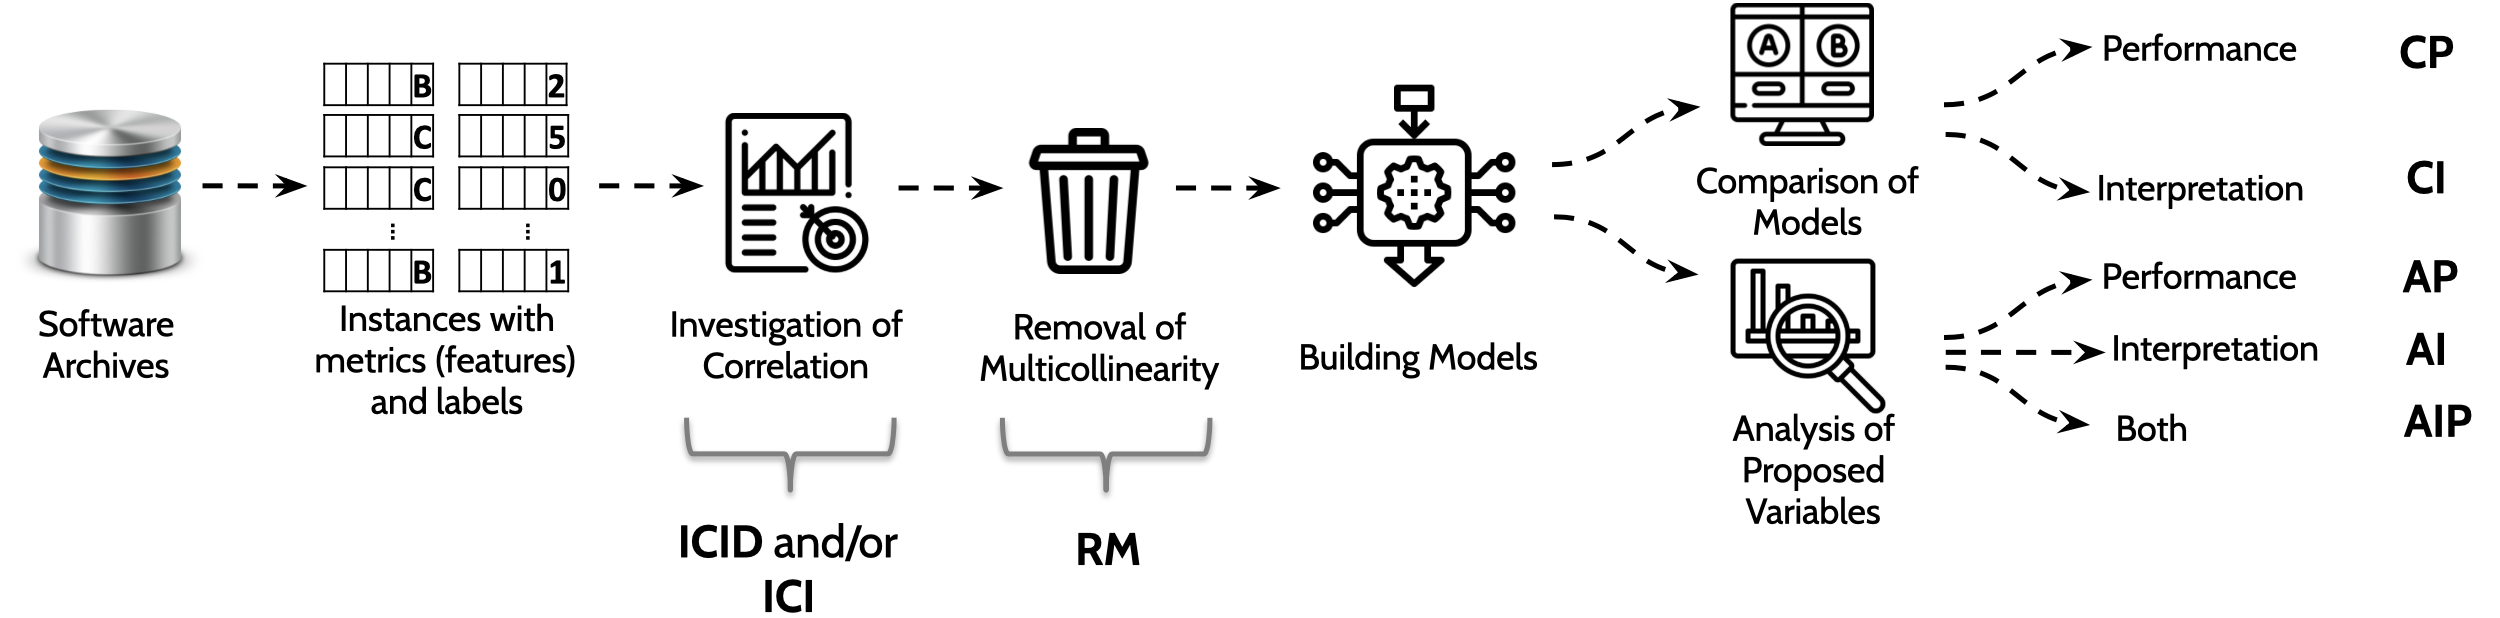
\includegraphics[width=\linewidth]{figures/eight_actions.png}
	\caption{The process of defect prediction studies with handling multicollinearity}
% 	\jc{Fix as Building models, Comparison of Models}}
	\label{fig:eight_actions}
\end{figure*}

The remainder of this paper is organized as follows. Section~\ref{sec:background} presents a theoretical discussion of multicollinearity and a literature survey of previous defect prediction studies relevant to this topic.
Sections~\ref{sec:experimentalsetup} and ~\ref{sec:result} design experiments based on research questions that can make clear how to deal with the multicollinearity issue in defect prediction studies and show the results of the experiments respectively. In Section~\ref{sec:discussion}, the experiment results are discussed in detail and practical guidelines for prediction model construction considering the multicollinearity problem are provided. The threats to validity of this study are also discussed. Finally, the study is summarized and concluded in Section~\ref{sec:conclusion}.
%irrelevancy and redundancy between features in the classification problems~\cite{Hall2003TKDEfeatureselection}.

\clearpage